\begin{figure*}[thb!]
  \caption{Approach overview}
  \centering
  \label{fig:approach}
  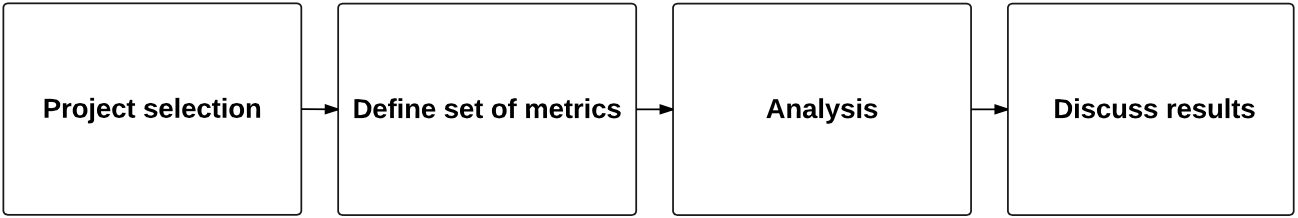
\includegraphics[width=1\textwidth]{figures/approach}
\end{figure*}

The goal of our project is to distinguish Defect Debt from Bugs. In order to do that we conducted a study using one large open source project, Google Chrome. We present our approach overview in figure \ref{fig:approach}. First, we extract data from the source code and from the issuer tracker repositories. Second,  we process the data to find relevant attributes and link them together. Third, we define our set of metrics. Then we analyze our results and answer the research questions. In the following sections we explain in details each one of the steps in our approach.   

\subsection{Data Extraction}

We use Google Chrome to conduct our study. Chrome is a large, mature open source software mostly written in C/C++. The criteria to select this project are its size, \peter{Don't use ease as a reason} the easy access to its source code repository and to the its issuer tracker. Other than that, we had at our disposal some of the desired data that was used in a previous study. \peter{you mean bug reports?} This data contained 47.938 html files and 5 tables. Each one of the files represent a bug extracted from the issue tracker. The tables contains the necessary information to link issues files, bugs and commits together. More details about the project can be found in table \ref{tab:project_details}.

To complement the data necessary to our study, we extract from the Chrome Releases website \cite{chrome_releases} the release date of each stable version release, the tag of the release and the release number. Then we store this data in our database.
 
In order to have all the source code available we clone Chromium Git repository. 

\begin{table*}[!hbt]
      \begin{center}
            \caption{Project details}
            \label{tab:project_details}
            \begin{tabular}{l| c c c c c}
            \toprule
            \textbf{Release}  & \textbf{Tag} & \textbf{Date} & \textbf{\# of commits} & \textbf{\# of Bug Reported} & \textbf{\# of Bug Fixed} \\ \midrule 
              1               & 1.0.154.36    & 2008-12-11   &    7705                &         1964                &      1014 \\
              2               & 2.0.172.28    & 2009-05-21   &    8015                &         3061                &      2493 \\
              3               & 3.0.195.21    & 2009-09-15   &    8583                &         4542                &      3669 \\
              4               & 4.0.249.78    & 2010-01-25   &    8045                &         3799                &      3710 \\
              5               & 5.0.375.55    & 2010-05-25   &    7603                &         3590                &      3464 \\
              6               & 6.0.472.53    & 2010-09-02   &    3457                &         1739                &      1696 \\
              7               & 7.0.517.43    & 2010-10-19   &    3376                &         1624                &      1423 \\
              8               & 8.0.552.215   & 2010-12-02   &    3990                &         1850                &      1703 \\
              9               & 9.0.597.84    & 2011-02-03   &    2703                &         1210                &      1191 \\
             10               & 10.0.648.127  & 2011-03-08   &    4671                &         1992                &      1833 \\
             11               & 11.0.696.57   & 2011-04-27   &    4083                &         1606                &      1587 \\
             12               & 12.0.742.91   & 2011-06-07   &    5198                &         2511                &      2263 \\
             13               & 13.0.782.107  & 2011-08-02   &    4541                &         1999                &      2082 \\
             14               & 14.0.835.163  & 2011-09-16   &    4077                &         2398                &      1840 \\
             15               & 15.0.874.102  & 2011-10-25   &    5505                &         2900                &      2814 \\
             16               & 16.0.912.63   & 2011-12-13   &    5036                &         3033                &      2670 \\
             17               & 17.0.963.46   & 2012-02-08   &    6624                &         3365                &      3775 \\
             18               & 18.0.1025.142 & 2012-03-28   &    5798                &         3537                &      3098 \\
             19               & 19.0.1084.52  & 2012-05-15   &    5395                &         2895                &      3141 \\
             20               & 20.0.1132.43  & 2012-06-26   &    3865                &         2211                &      2174 \\
             21               & 21.0.1180.57  & 2012-07-31   &    7187                &         4012                &      4337 \\
             22               & 22.0.1229.79  & 2012-09-25   &    5247                &         2808                &      2927 \\
             23               & 23.0.1271.83  & 2012-11-02   &    7967                &         4108                &      4614 \\
             24               & 24.0.1312.52  & 2013-01-10   &    5707                &         2753                &      3541 \\
             25               & 25.0.1364.97  & 2013-02-21   &    5009                &         2129                &      3019 \\ \bottomrule
            \end{tabular}
      \end{center}
\end{table*}

\subsection{Process data and find attributes}

After the extraction we process the data and search for attributes that will help us in our analysis. 

First, we create the attributes to store the date that the bug was reported, the release which the bug was reported, the number of comments found in the bug and the release that the bug was commited. Then we process the issues files to get the reported date and the number of comments of each bug. The release and commit dates we get from the release table. 

Second, we create the attributes to store information about the commit classification and the files included in the commit. We use Commit Guru\cite{commit_guru} to gather this information. Commit Guru is an on-line tool, which run a series of source code analysis in a given git repository url. The commit classification is based on the commit message and is used to predict the intend of a change. The process uses key words and expressions that are strong indicators of intend, like `add' or `bug fix'. The possibles classifications are `Feature Addition', `Corrective', `Preventative', `Merge', `Non Functional', `Perfective' and without classification.

Third, we create a table to store metrics values. We collect our metrics using Understand a code analysis tool. This tool can analyze different releases of a project and create a separated database containing several metrics \cite{understand_metrics} for each one of the processed releases. It is possible to access these databases through an API and collect the processed information. We checkout 18 stable releases from our Chrome repository based on the collected tag information from the selected releases. Due to the size of the project and time constraints we use only the `chrome' directory without the third party libraries in our analysis. The whole process took approximately 16 hours and generated more than 2GB of data. 

Different scripts written in Python and SQL were developed during this study in order to make this process automatic and easily reproducible. We provide the link\footnotetext{https://github.com/maldonado/soen6611} to these files just to evaluation purposes.

\subsection{Link data}

The most important data to link for our study are bug reports and the commits that are addressing them. As mentioned before, we took advantage of data used in a different study that had done this work already. Other than that, we link all of our entities in the database with releases as we are investigating the behavior of Defect Debt and Bugs per release. 

\subsection{Define metrics}

In this section we describe the metrics used in our study. All of the metrics are grouped by release as our goal is to analyze the project in the release level. 

\textbf{Commit classification:} A commit can be classified as `Feature Addition', `Corrective', `Preventative', `Merge', `Non Functional', `Perfective' and without classification. We store the total number of each one of these classifications per release. 

\textbf{Churn:} We calculate churn as the number of lines changed in a file compared with its previous version. Both the addition and deletion of a line in a file is considered as a change. We calculate the total churn by summing the number of lines added and removed of all commits per release. \peter{This sounds strange, are you just counting +/- in a diff?}

\textbf{Developers:} This metric is the number of developers that had at least one commit in the analyzed version. In our study a developer is identified by the user login contained in the commit message. We choose to identify the developers by the login instead of using email because most developers have more than one email account in their git account. \peter{ok, may need to validate this later}

\textbf{Developers joining or leaving the project:} This is a derived metric based on the total number of developers in the previous release. If the difference of unique developers from one release to another is positive we store this value as developers joining, and if the difference is negative we store the value as developers leaving the project. We do not make any assumption of the experience of the developers in this metric.

\textbf{Complexity:} This metric is McCabe's Cyclomatic Complexity \cite{mccabeTSE1976} calculated by Understand tool.

\textbf{Lines of code:} The count of all lines of code in the source files including comments. This metric does not take into consideration blank lines.

\textbf{Bug report comments:} We extract this metric based on the number of replies that one posted bug report has. All replies in the issuer tracker is treated as a comment. Our perception is that users impacted by a Defect Debt will comment in the issuer tracker page to ask for a fix or to search for a `work-around' while the problem is not solved. We intuitively think that bug reports with a hight number of comments are bug reports of Defect Debt.
\peter{Haven't you done past work on this? I didn't see this in the background}

\textbf{Bug report next to new release:} This metric is the total number of bug reports created close to next release date. We use a threshold of 2 weeks to calculate this metric.  

\textbf{Total number of files changed:} This is the total number of files that were changed in the current analyzed version. 

 We selected these metrics based on the analysis of our three research questions that we cover in detail in the next section.

